% Template for ICASSP-2018 paper; to be used with:
%          spconf.sty  - ICASSP/ICIP LaTeX style file, and
%          IEEEbib.bst - IEEE bibliography style file.
% --------------------------------------------------------------------------
\documentclass{article}
\usepackage{spconf,amsmath,graphicx}

% Example definitions.
% --------------------
\def\x{{\mathbf x}}
\def\L{{\cal L}}

% Title.
% ------
\title{SINGLE SOURCE AUDIO SEPARATION}
%
% Single address.
% ---------------
\name{Author(s) Name(s)\thanks{Thanks to XYZ agency for funding.}}
\address{Author Affiliation(s)}
%
% For example:
% ------------
%\address{School\\
%	Department\\
%	Address}
%
% Two addresses (uncomment and modify for two-address case).
% ----------------------------------------------------------
%\twoauthors
%  {A. Author-one, B. Author-two\sthanks{Thanks to XYZ agency for funding.}}
%	{School A-B\\
%	Department A-B\\
%	Address A-B}
%  {C. Author-three, D. Author-four\sthanks{The fourth author performed the work
%	while at ...}}
%	{School C-D\\
%	Department C-D\\
%	Address C-D}
%
\begin{document}
%\ninept
%
\maketitle
%
\begin{abstract}
In this paper we propose a Deep Attractor  based audio separation method from single sources.
\end{abstract}
%
\begin{keywords}
Single Source Audio Separation, Deep Attractor, Wasserstein GAN
\end{keywords}
%
\section{Introduction}
\label{sec:intro}



\section{Related work}
\label{sec:related}
\subsection{LSTM Denoising Autoencoder feature-mapping network }
Previous works have used the Long-Short Term Memory (LSTM) denoising autoencoders, which has 
shown better performance than feature-mapping networks. A disadvantage of this method is that it requires
a fixed number of sources. 
\subsection{Deep clustering-based separator}
DC can solve both permutation and output dimension problem to produce the state of the art separation performance. 
However, the main drawback of DC is its inefficiency to perform end-to-end mapping, because the objective function is the affinity between the sources in the embedded space and not the separated signals themselves. Minimizing the separation error is done with an unfolding clustering system and a second network, which is trained iteratively and stage by stage to ensure convergence.

\section{Model design}
\label{sec:format}
\begin{figure}[htb]

\begin{minipage}[b]{1.0\linewidth}
  \centering
  \centerline{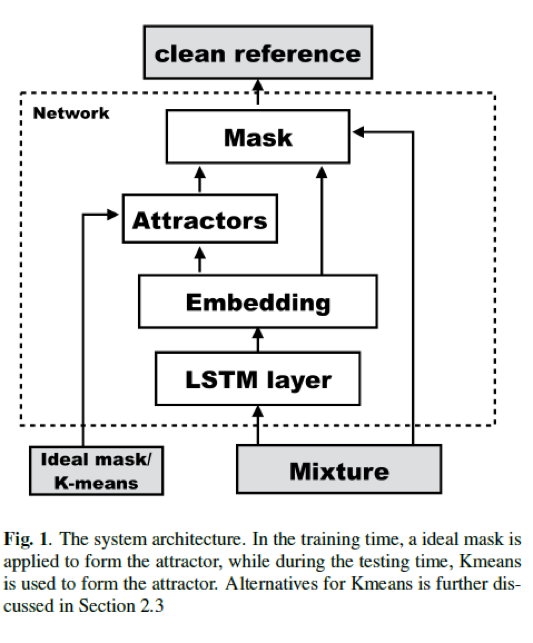
\includegraphics[width=8.5cm]{Picture1.png}}
%  \vspace{2.0cm}
  \centerline{(a) Result 1}\medskip
\end{minipage}
%
\caption{System architecture.}
\label{fig:res}
%
\end{figure}


\section{Data Collection }
\label{sec:pagestyle}

It contains a 30 h training set and a 10 h validation set generated by randomly selecting utterances from
different speakers in the Wall Street Journal (WSJ0) training set sitrs, and mixing them at various signal-to-noise ratios (SNR) randomly chosen between 0 dB and 10 dB.

\section{Experimentation}
\label{sec:typestyle}



\section{Evaluation}
\label{sec:majhead}



\section{Conclusion}
\label{sec:print}



\vfill\pagebreak

\section{References}
\label{sec:refs}



% References should be produced using the bibtex program from suitable
% BiBTeX files (here: strings, refs, manuals). The IEEEbib.bst bibliography
% style file from IEEE produces unsorted bibliography list.
% -------------------------------------------------------------------------
\bibliographystyle{IEEEbib}
\bibliography{strings,refs}

\end{document}
